%%%%%%%%%%%%%%%%%%%%%%%%%%%%%%%%%%%%%%%%%%%%%%%%%%%%%%%%%%%%%%%%%%%%%%%%%%%%% 
%
% This is a LaTeX file for an A0 poster.
% 
% template poster taken from https://canizo.org/latex_poster
%
%%%%%%%%%%%%%%%%%%%%%%%%%%%%%%%%%%%%%%%%%%%%%%%%%%%%%%%%%%%%%%%%%%%%%%%%%%%%% 

%%%%%%%%%%%%%%%%%%%%%%%%%%%%%%%%%%%%%%%%%%%%%%%%%%%%%%%%%%%%%%%%%%%%%%%%%%%%% 
%%%%%%%%%%%%%%%%%%%%%%%%%%%%%%%%%%%%%%%%%%%%%%%%%%%%%%%%%%%%%%%%%%%%%%%%%%%%%
%
% Towards a standardized workflow for mass spectrometry based single-cell 
% proteomics
%
% Poster for the Applied Bioinformatics for Life Science, February 2020, Leuven.
%
%%%%%%%%%%%%%%%%%%%%%%%%%%%%%%%%%%%%%%%%%%%%%%%%%%%%%%%%%%%%%%%%%%%%%%%%%%%%%
%%%%%%%%%%%%%%%%%%%%%%%%%%%%%%%%%%%%%%%%%%%%%%%%%%%%%%%%%%%%%%%%%%%%%%%%%%%%%

\documentclass{article}
% To modify the size of the page:
\usepackage[dvips,a3paper,portrait,centering,margin=0.5cm]{geometry}
% To create multiple columns
\usepackage{multicol}

\usepackage[utf8]{inputenc}
% To align images
\usepackage[export]{adjustbox}
% Use captions in minipages
\usepackage{caption}
% Math font
\usepackage{amsmath, amsthm, amsfonts}
% Include figure files.
\usepackage{graphicx}

% Coding fonts
% ------------
% For including R chunks 
\usepackage{listings} 
\lstset{
  language=R,
  basicstyle=\footnotesize\ttfamily\color{vdgray}, % the size of the fonts that are used for the code
  % sensitive=false,
  numbers=left,                   % where to put the line-numbers
  numberstyle=\tiny\color{gray},  % the style that is used for the line-numbers
  stepnumber=1,                   % the step between two line-numbers.
  numbersep=0.1cm,                % how far the line-numbers are from the code
  backgroundcolor=\color{lgray},  % choose the background color. You must add \usepackage{color}
  deletekeywords={stat},
  keywordstyle=\color{blue},      % keyword style
  stringstyle=\color{green},      % string literal style
  xleftmargin=0.5cm,
}
% Create command for highlighting inline code or variables
\newcommand{\hcode}[2][lgray]{{\ttfamily\color{vdgray}\colorbox{#1}{#2}}}

% Colors
% ------
\usepackage{color}
\usepackage[dvipsnames]{xcolor}
% Color panel used throughout the poster
\definecolor{lgray}{rgb}{0.9179688,0.9179688,0.9179688} % #ebebeb
\definecolor{dgray}{rgb}{0.796875,0.796875,0.796875} % #cccccc
\definecolor{vdgray}{rgb}{0.3984375,0.3984375,0.3984375} % #666666
\definecolor{coral}{rgb}{0.9960938,0.4960938,0.3125000} % #ff7f50
\definecolor{blue}{rgb}{0.4218750,0.6484375,0.8007812} % #6ca6cd
\definecolor{green}{rgb}{0.6992188,0.7265625,0.5078125} % #b3ba82
\definecolor{yellow}{rgb}{0.9570312,0.8671875,0.6992188} % #f5deb3

% Bibliography
% ------------
\usepackage{url}
% Adjust space between reference items
\let\OLDthebibliography\thebibliography
\renewcommand\thebibliography[1]{
  \OLDthebibliography{#1}
  \setlength{\parskip}{0pt}
  \setlength{\itemsep}{0pt plus 0.3ex}
}
  
\pagestyle{empty}

\def\to{\rightarrow}


% ===========================================================================

\title{}
\author{}
\date{}

\begin{document}


% ---------------------------------------------------------------------------
% Banner


\begin{center}
\colorbox{lgray}{
  \begin{minipage}{3.7cm}
    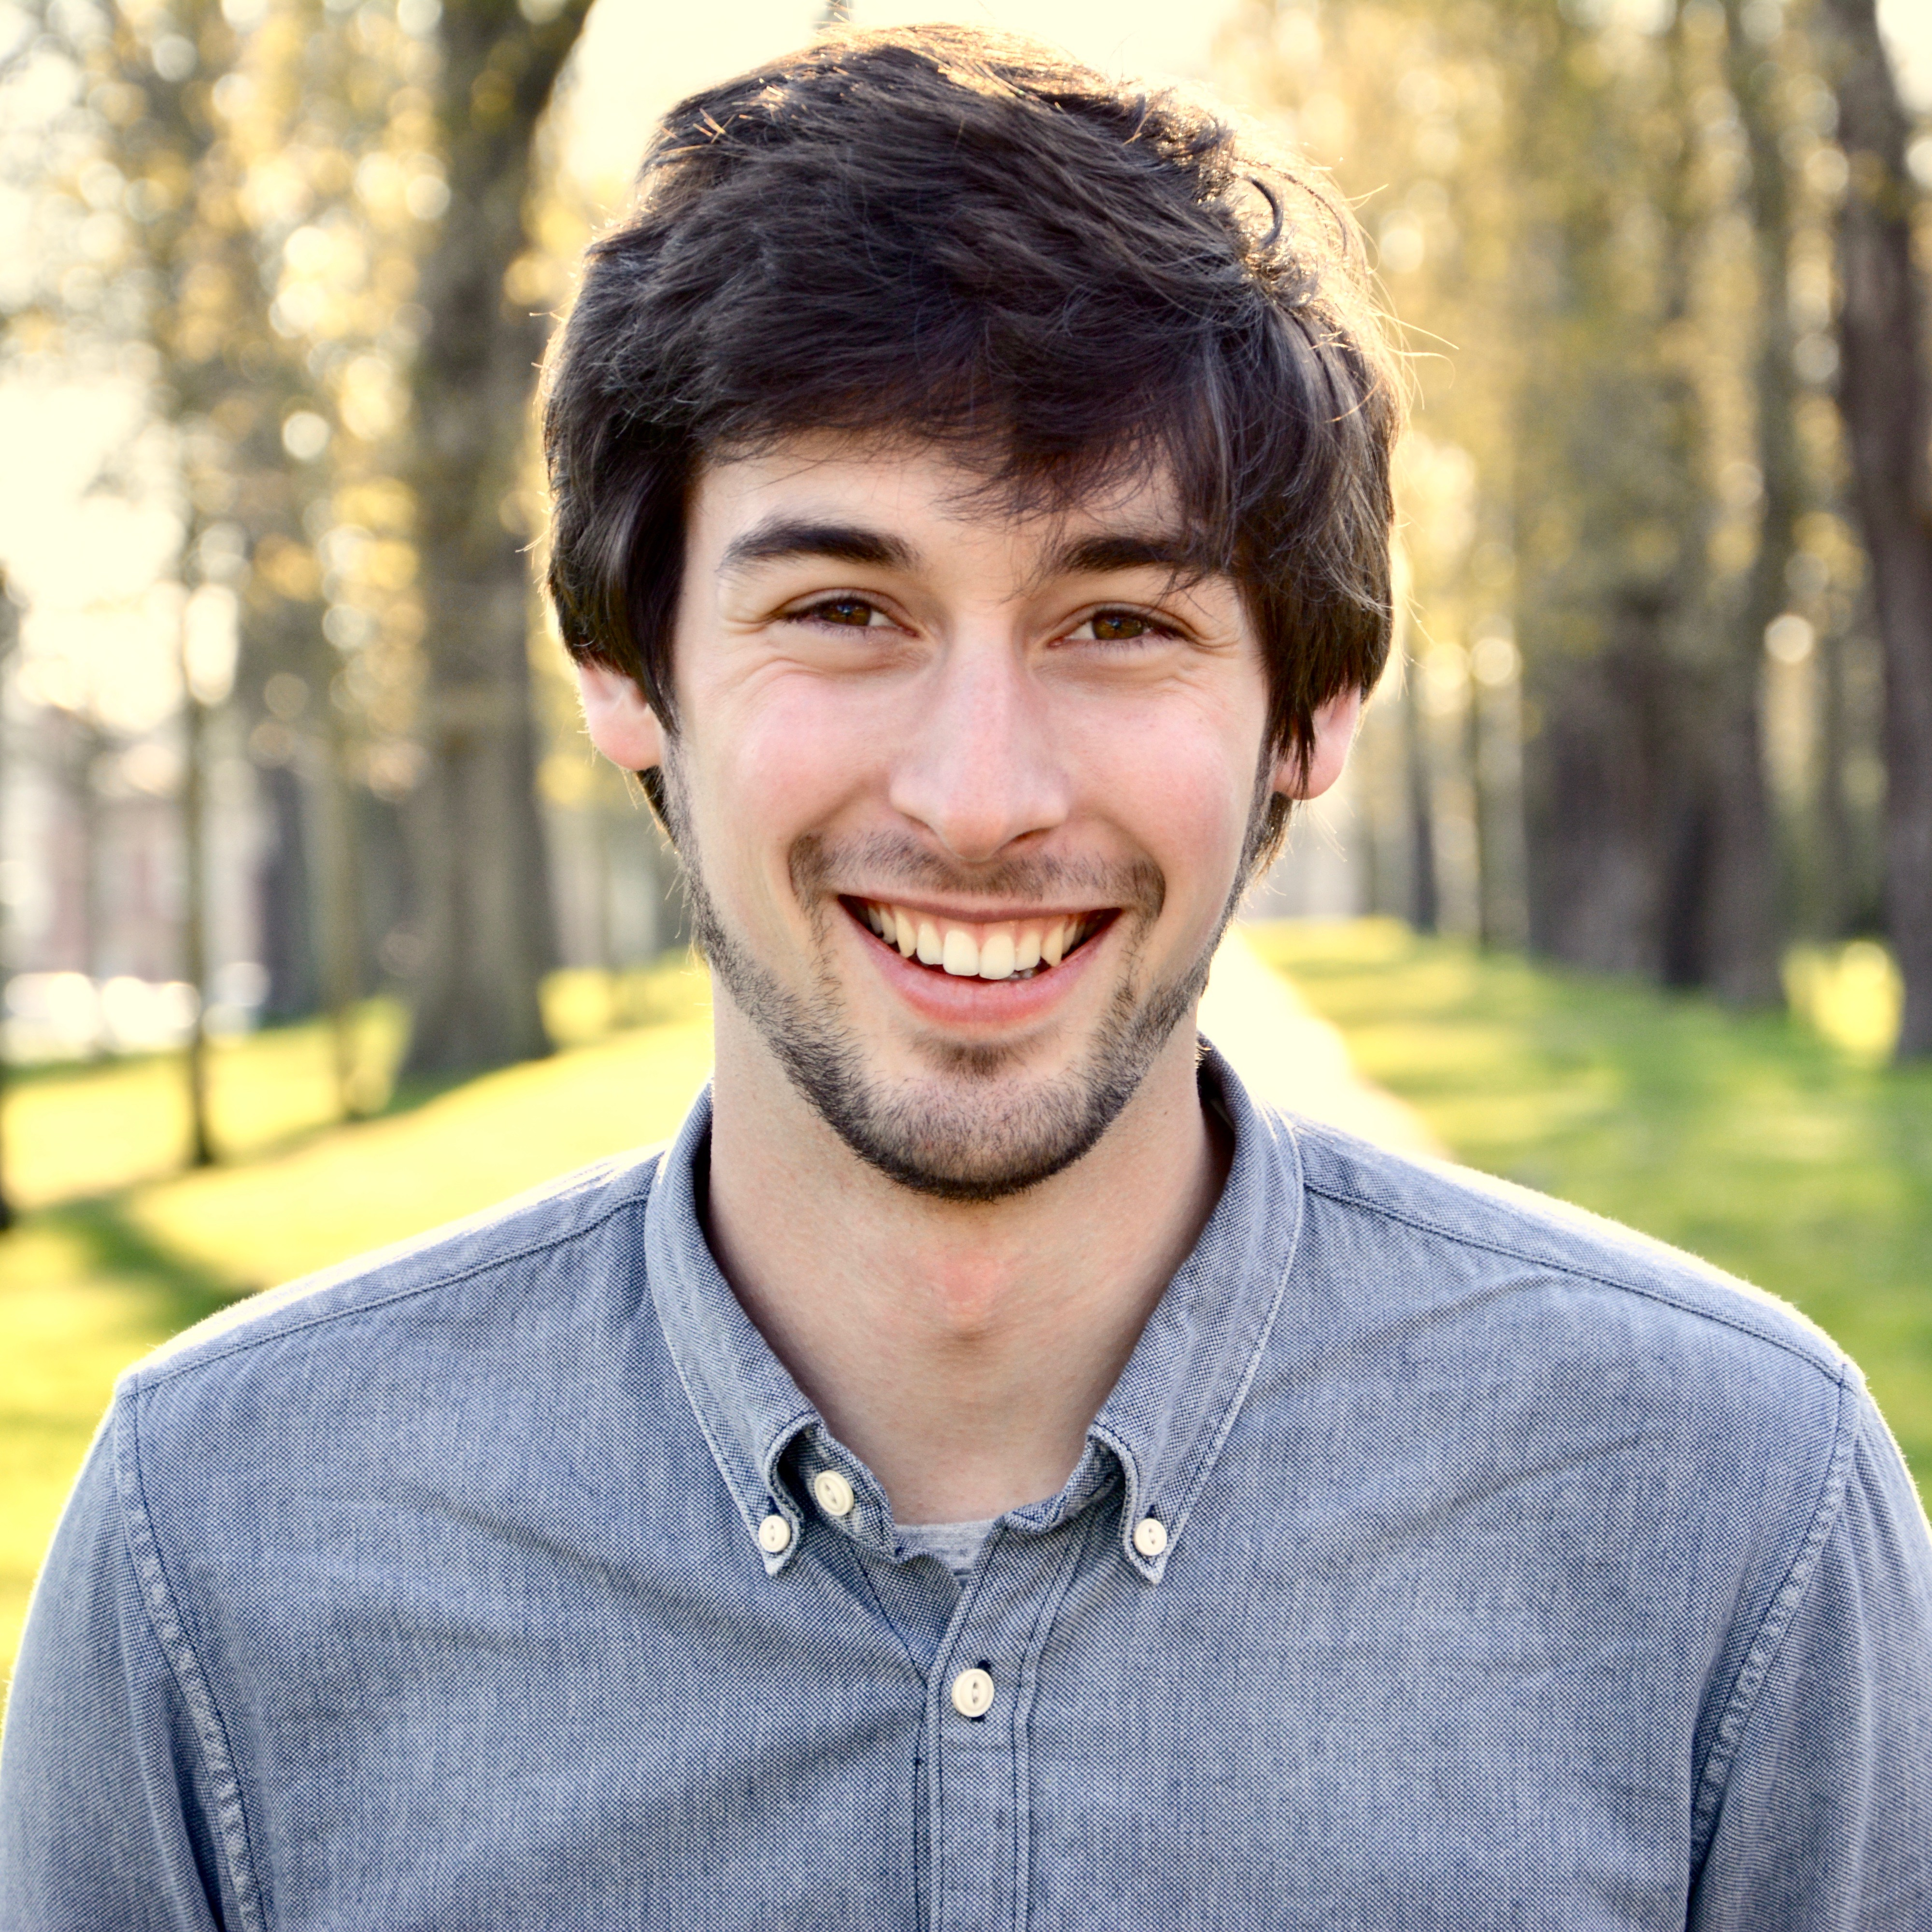
\includegraphics[width=1.2\linewidth]{figs/DSC_2812.jpg}
  \end{minipage}
  %&
  \begin{minipage}{.72\textwidth}
    \begin{center}
      % Title 
      \vspace{0.4cm}
      \huge 
      \hspace{1cm}
      \noindent
      \textbf{Towards a standardized workflow for mass spectrometry-based single-cell proteomics} \\
      \vspace{0.4cm}
      % Authors
      \Large \textbf{Christophe Vanderaa, Laurent Gatto} \\
      % Affiliation
      \Large \textit{Computational biology and bioinformatics, de Duve Institute, UCLouvain } \\
      % email
      \vspace{0.4cm}
      \normalsize christophe.vanderaa@uclouvain.be \\
      \hspace{1cm}
    \end{center}
  \end{minipage}
  %&
  \begin{minipage}{3.7cm}
      \includegraphics[width=0.7\linewidth, right]{figs/fnrs.png} \\
      \vspace{0.5cm}
      \includegraphics[width=1.1\linewidth, right]{figs/ucl.png}
  \end{minipage}
}
\end{center}


% ---------------------------------------------------------------------------
% Summary + conclusion
\noindent
% Summary
\colorbox{yellow}{
  \noindent
  \begin{minipage}[t]{13.7cm}
  \vspace{.15cm}
    \section*{\huge Summary}
    \large 
    Recent advances in sample preparation, processing and mass spectrometry (MS) have allowed the emergence of MS-based \textbf{single-cell proteomics} (SCP). We are currently developing a \textbf{workflow} for analyzing MS-SCP data. It relies on a \textbf{standardized} data structure combining Bioconductor classes used for singe-cell analyses, \textbf{\hcode[yellow]{SingleCellExperiment}}\cite{SCE}, and for MS-based proteomics analyses, \textbf{\hcode[yellow]{Features}}\cite{Features}, facilitating re-use of current state-of-the-art software.
    \vspace{0.1cm}
  \end{minipage}
}
\hspace{0.37cm}
% Conclusion
\noindent
\colorbox{yellow}{
  \begin{minipage}[t]{13.6cm}
    \vspace{.2cm}
    \section*{\huge Conclusion}
    \large
    MS-based SCP is still in its infancy. Nevertheless, the amount of available data is rapidly increasing and so is the need for dedicated analysis software. We designed a \textbf{standardized workflow} compatible with the current MS-SCP technologies. The data structure allows \textbf{easy integration} of currently available software for data analysis and visualization. It will also facilitate development of dedicated algorithms for dealing with \textbf{missing data} and \textbf{batch effects} that are characteristic of MS-SCP data.
    \vspace{0.15cm}
 \end{minipage}
}
\vspace{-1cm}


% ---------------------------------------------------------------------------
% Create a 2 column layout
\setlength{\columnsep}{0.5cm}
\begin{multicols}{2}

% ---------------------------------------------------------------------------
% MS-SCP technologies
\noindent
\begin{minipage}[t]{\linewidth}
  \vspace{0.5cm}
  \section*{\huge MS-SCP technologies}
  \large
  \textbf{\large nanoPOTS pipeline} (Zhu et al., 2018, \cite{Zhu2018-bf}) runs label-free proteomics for single cells. The \textbf{\color{BrickRed}{throughput is low}} ($\pm$ 10 samples/day), but it achieves \textbf{\color{OliveGreen}{accurate peptide quantification}}. Identification is improved using information between runs. 
  \vspace{-0.3cm}
  \begin{center}
    \includegraphics[width=0.87\linewidth]{figs/nanopots.png} \\
  \end{center}
  
  \textbf{\large SCoPE2 pipeline} (Specht et al., 2019, \cite{Specht2019-jm}) adapts TMT-based proteomics to single-cells. The \textbf{\color{OliveGreen}{throughput is higher}} ($\pm$ 5 samples/hour), but it suffers from \textbf{\color{BrickRed}{batch effects}}. Identification is improved using a data-driven Bayesian framework.
  \vspace{-0.3cm}
  \begin{center}
    \includegraphics[width=0.9\linewidth]{figs/scopems.png} \\
  \end{center}
  
  \textbf{\large Both methods} generate data containing a high rate of \textbf{\color{BrickRed}{missing values}}.
    
\end{minipage}

% ---------------------------------------------------------------------------
% Data structure
\noindent
\begin{minipage}[t]{\linewidth}
  \vspace{0.55cm}
  \section*{\huge Data Structure}
  \begin{center}
    \includegraphics[width=0.92\textwidth, trim={2.6cm 5cm 13.7cm 1cm},clip]{figs/Features.pdf}
  \end{center}
  % \hspace{3.5cm} \includegraphics[width=0.7\textwidth]{figs/annexinA2.png}
\end{minipage}


% ---------------------------------------------------------------------------
% Data manipulation
\noindent
\begin{minipage}[t]{\linewidth}
  \vspace{0.55cm}
  \section*{\huge Data manipulation}
  \large
  We implemented standardized functions to reproduce part of the analysis from \cite{Specht2019-jm}, integrating functionality from \hcode{Features} and \hcode{SingleCellExperiment}.
  \begin{lstlisting}
  sce <- SingleCellExperiment(assays = list(assayDat), 
                              rowData = rowDat,
                              colData = colDat)
  Features(experiments = list(peptide = sce), 
           colData = colData(sce_pep)) %>%
    scp_normalizeFeatures("peptide", name = "peptide_norm",
                          FUN = "mean", na.rm = TRUE)  %>%
    scp_aggregateFeatures("peptide_norm", name = "protein"
                          fun = colMeans, na.rm = TRUE,
                          fcol = "ProteinAccession")  %>%
    scp_normalizeFeatures("protein", name = "protein_fnorm"
                          FUN = "mean", na.rm = TRUE) %>%
    scp_normalizeSamples("protein_fnorm", name = "protein_snorm"
                         FUN = "median", na.rm = TRUE, ) %>%
    scp_impute("protein_fnorm", name = "protein_imputed"
               method = KNNimputation, k = 3) %>%
    scp_batchCorrect("protein_imputed", name = "protein_batchCorrected",
                     batch = "raw.file", target = "celltype") -> 
    fts
  \end{lstlisting}
\end{minipage}

% ---------------------------------------------------------------------------
% Data visualization
\noindent
\begin{minipage}[t]{\linewidth}
  \vspace{0.5cm}
  \section*{\huge Data visualization}
  \large
  Data can directly be analyzed by packages dedicated to the \hcode{SingleCellExperiment} class. For instance, we performed dimension reduction using the \hcode{scater} package. 
  \begin{center}
    \includegraphics[width=0.8\textwidth, trim={0 0 0 0}, clip]{figs/dimred.png}
  \end{center}
  Feature expression data can easily be extracted accross different levels using the \hcode{Features} data structure.
  \begin{lstlisting}
    stat3 <- fts["P42227-2", , ]
  \end{lstlisting}
  \vspace{-0.5cm}
  \begin{center}
  \includegraphics[width=0.8\textwidth, trim={0 0 0 0}, clip]{figs/Stat.png}
  \end{center}
  
\end{minipage}

% ---------------------------------------------------------------------------
% Problems to tackle
\noindent
\begin{minipage}[t]{\linewidth}
  \section*{\huge Problems to tackle}
  \vspace{0.1cm}
\end{minipage}
% Left column
\begin{minipage}[t]{0.45\linewidth}
  \large
  \textbf{Batch effects} \normalsize are inherent to MS-SCP data since many samples have to be distributed across \textbf{different MS runs}, in particular for TMT-based proteomics where every run contains a small group of cells.
  \begin{center}
    \includegraphics[width=\linewidth, trim={2cm 9cm 2cm 3.5cm},clip]{figs/batchEffect.png}
  \end{center}
\end{minipage}
% Right column
\hspace{1cm}
\begin{minipage}[t]{0.45\linewidth}
  \large
  \textbf{Missing data}: \normalsize MS-SCP data is very sparse for \textbf{biological} reasons (\textit{e.g.} some proteins are not expressed in all cells) and for \textbf{technical} reasons (low amounts of sample material, instrument sensitivity and batch effects).
  \begin{center}
    \includegraphics[width=0.85\linewidth, trim={0 2cm 0 0}]{figs/missing.png} \\
    \vspace{0.5cm}
    \includegraphics[width=0.6\linewidth, trim={2cm 3cm 0cm 3.8cm},clip]{figs/missing-leg.png}
  \end{center}
  \vspace{0.4cm}
\end{minipage}


% ---------------------------------------------------------------------------
% Additional notes
\noindent
This work is funded by an Aspirant FRS-FNRS fellowship awarded to Christophe Vanderaa. The poster is available at {\color{blue}{https://github.com/cvanderaa/ABLS2020-Poster}}.

% ---------------------------------------------------------------------------
% References
\scriptsize
\bibliography{ref.bib} 
\bibliographystyle{ieeetr}

% ---------------------------------------------------------------------------
% End of poster
\end{multicols}
\end{document}